%%%%%%%%%%%%%%%%%%%%%%%%%%%%%%%%%%%%%%%%%
%
% (c) 2018 by Jennifer Laaser
%
% This work is licensed under the Creative Commons Attribution-NonCommercial-ShareAlike 4.0 International License. To view a copy of this license, visit http://creativecommons.org/licenses/by-nc-sa/4.0/ or send a letter to Creative Commons, PO Box 1866, Mountain View, CA 94042, USA.
%
% The current source for these materials is accessible on Github: https://github.com/jlaaser/pogil-polymers
%
%%%%%%%%%%%%%%%%%%%%%%%%%%%%%%%%%%%%%%%%%

\section{Degree of Polymerization in Step-Growth Polymerizations}
\renewcommand{\figpath}{content/polymchem/stepgrowth/Mn-and-stoich/figs}

%\textbf{Focus question:} Put a central question for the students to consider through this exercise here.

\subsection{Model 1:  Polymerization of ``AB''-Type Monomers}

The simplest type of step-growth polymerization is one in which each monomer has one ``A''-type reactive group and one ``B''-type reactive group.
These types of monomers are referred to as ``AB''-type monomers.

In each step of the polymerization, an ``A'' group on one molecule reacts with a ``B'' group on another molecule to form an ``ab'' bond, as shown below:

\vspace{0.1in}
\centerline{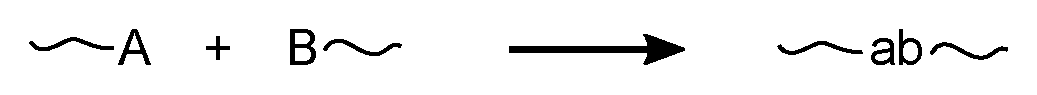
\includegraphics[width=0.6\textwidth]{\figpath/ABrxn.pdf}}

For example, for a simple reaction mixture containing 8 ``AB''-type monomers, the evolution of the reaction mixture might look something like this:

\vspace{0.1in}
\centerline{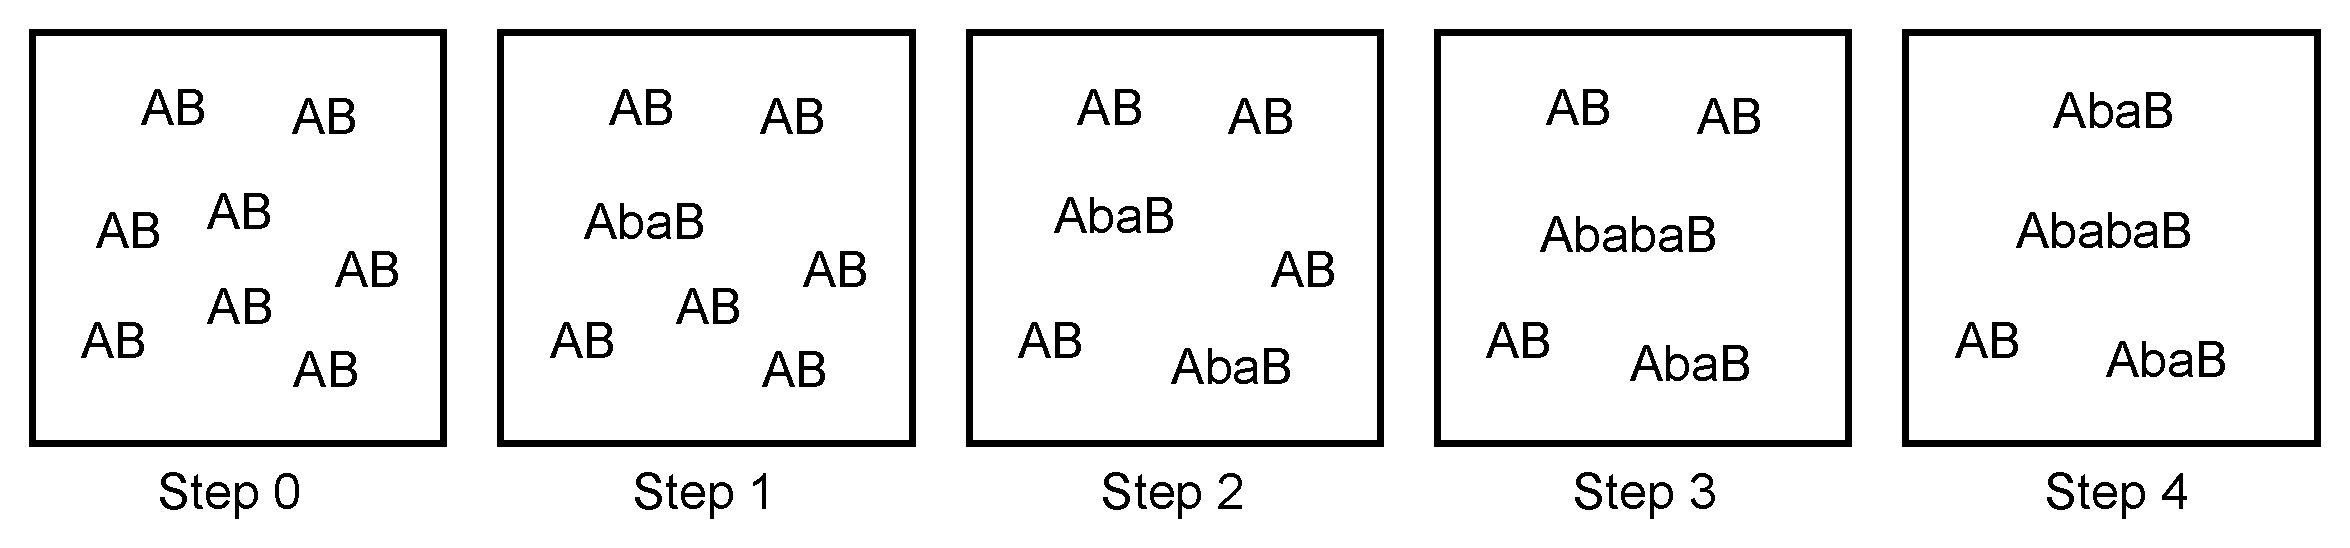
\includegraphics[width=0.9\textwidth]{\figpath/ABpolym.pdf}}

% to include images, put them in the folder specified by figpath and then use:
%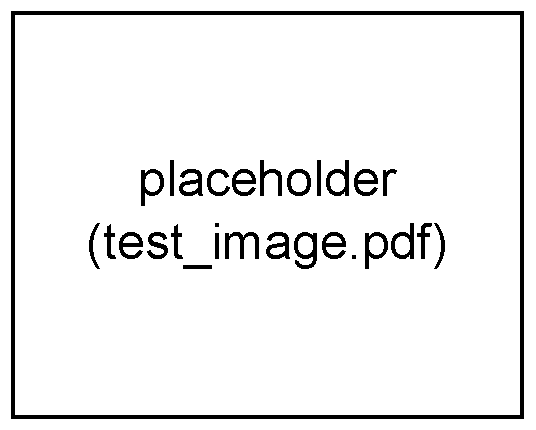
\includegraphics[width=0.8\textwidth]{\figpath/test_image.pdf}

\subsection*{Critical Thinking Questions}

	\begin{enumerate}
		\item \label{ctq:ABtable} For the reaction mixture shown in Model 1, fill out the following table:
		
			\begin{table}[h]
				\centering
				\renewcommand{\arraystretch}{3}
				\begin{tabular}{|c|c|c|}
					\hline
					\textbf{Step} &  \textbf{Number of unreacted ``A'' groups} & \textbf{Number of molecules} \\\hline
					0 && \\\hline
					1 && \\\hline
					2 && \\\hline
					3 && \\\hline
					4 && \\\hline
				\end{tabular}
			\end{table}
		
		\clearpage
		\item Explain, in a complete sentence, how the number of molecules in the mixture is related to the number of unreacted ``A'' groups.
		
		\vspace{1in}
		
		\item The number-average degree of polymerization, $N_n$, is the total number of \emph{monomers} divided by the total number of \emph{molecules}.  Remembering that we started with 8 monomers, calculate the number-average degree of polymerization for each step shown in Model 1.
		
			\begin{table}[h]
				\centering
				\renewcommand{\arraystretch}{3}
				\begin{tabular}{|c|c|c|c|c|c|}
					\hline
					\textbf{~~Step~~} &  \textbf{~~~~0~~~~} & \textbf{~~~~1~~~~} & \textbf{~~~~2~~~~} & \textbf{~~~~3~~~~} & \textbf{~~~~4~~~~} \\\hline
					$\mathbf{N_n}$ &&&&& \\\hline
				\end{tabular}
			\end{table}
		
		\item Suppose that you had initially started with 100 monomers.  Then, suppose that at some time later, you had only 8 unreacted ``A'' groups left.
		
			\begin{enumerate}
				\item How many molecules would there be in the reaction mixture at this point?
				
				\item What would the number-average degree of polymerization be at this point?
			\end{enumerate}
			
		\item More generally, suppose you started with $v_A^0$ monomers, and at some time later, you had only $v_A$ unreacted ``A'' groups left.  What would the number average-degree of polymerization be at this point, in terms of $v_A^0$ and $v_A$?
		
		\vspace{1in}
		
	\end{enumerate}
	
	INFORMATION: Usually, we find it more useful to work in terms of the \emph{fraction} of all ``A'' groups that have reacted, rather than the total \emph{number} of ``A'' groups that have reacted.  In step-growth polymerizations, we refer to the fraction of ``A'' groups that have reacted as the ``extent of reaction'', $p$.
	
	\begin{enumerate}[resume]
		\item If we start with $v_A^0$ ``A'' groups, how many of the ``A'' groups will have \emph{reacted} when the extent of reaction is equal to $p$?
		
		\vspace{1in}
		
		\item How many ``A'' groups are still \emph{unreacted} when the extent of reaction is equal to $p$?
		
		\vspace{1in}
		
		\item Using your answers to critical thinking questions 5, 6, and 7, derive an expression for $N_n$ in terms of $p$.
		
		\vspace{1in}
		
	\end{enumerate}

\subsection{Model 2: Polymerization of ``AA'' and ``BB''-Type Monomers}

Now, let's consider a slightly more complicated reaction, with two different types of monomers that each have \emph{either} two ``A'' reactive groups \emph{or} two ``B'' type reactive groups.
We call monomers with two ``A'' groups ``AA''-type monomers, and we call monomers with two ``B'' groups ``BB''-type monomers.

Suppose we start with 4 ``AA''-type monomers and 4 ``BB''-type monomers.
In this case, the evolution of the reaction mixture might look something like this:

\vspace{0.1in}
\centerline{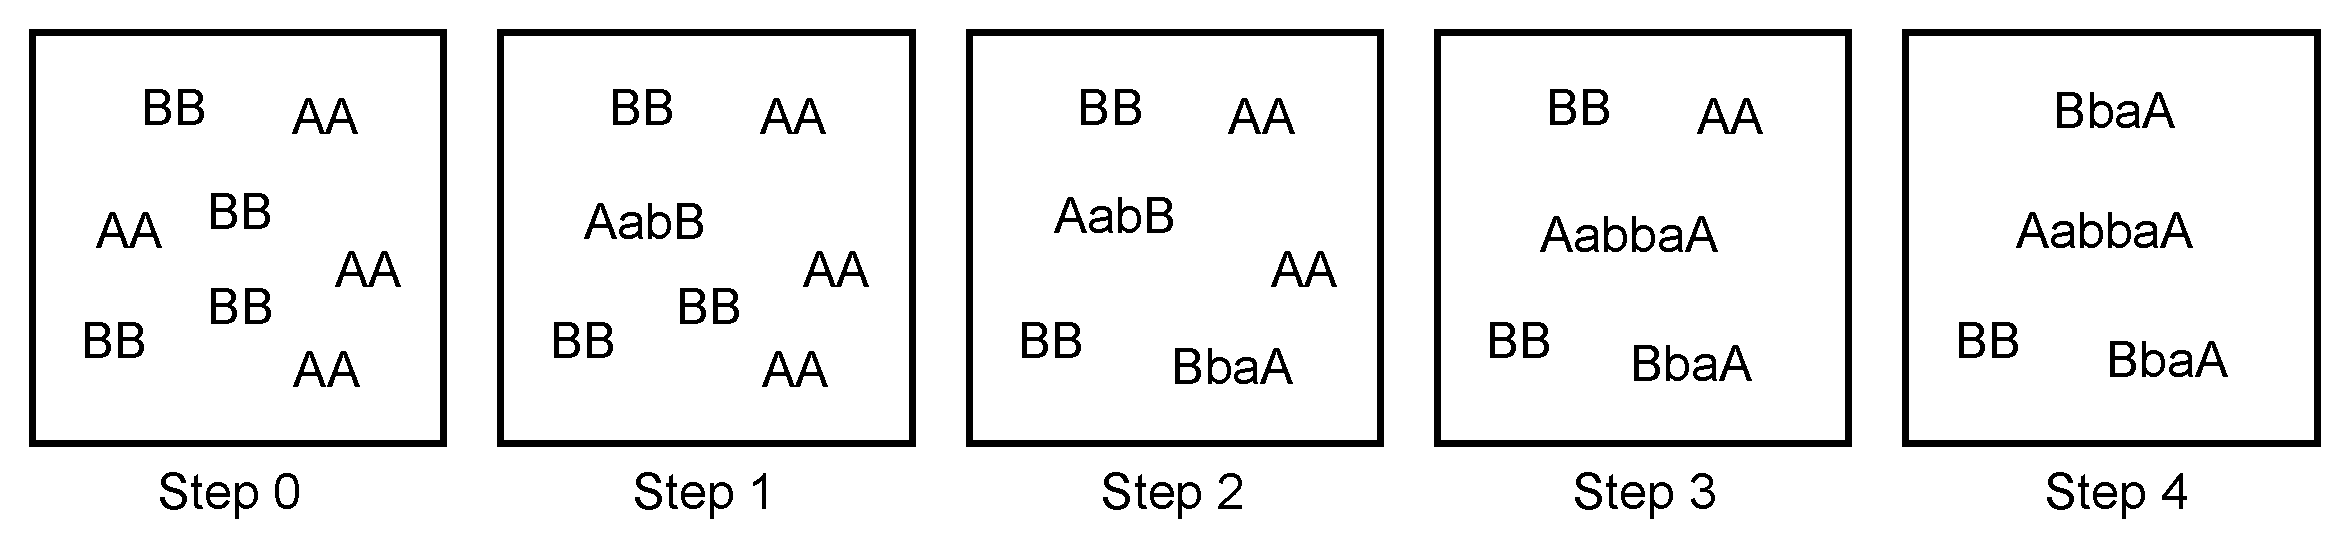
\includegraphics[width=0.9\textwidth]{\figpath/AABBpolym.pdf}}

\subsection*{Critical Thinking Questions}

	\begin{enumerate}[resume]
		\item \label{ctq:AABBtable} For the reaction mixture shown in Model 2, fill out the following table:
		
			\begin{table}[!h]
				\centering
				\renewcommand{\arraystretch}{3}
				\begin{tabular}{|c|c|c|c|}
					\hline
					\textbf{Step} &  \textbf{Number of unreacted ``A'' groups} & \textbf{Number of molecules} & ~~~~$\mathbf{N_n}$~~~~\\\hline
					0 &&& \\\hline
					1 &&& \\\hline
					2 &&& \\\hline
					3 &&& \\\hline
					4 &&& \\\hline
				\end{tabular}
			\end{table}
			
		\item Compare your answers in question \ref{ctq:AABBtable} with those from question \ref{ctq:ABtable}.  What similarities and/or differences do you notice?
		
		\vspace{1in}
		
		\item Consider the following statement:
		
			\emph{``In polymerizations of AA- and BB-type monomers, we should be able to use the same expressions to calculate $N_n$ as we did for polymerizations of AB-type monomers.''}
			
			In two or three complete sentences, briefly critique or defend this statement, making sure to explain your reasoning.
		
		\vspace{1.5in}
			
	\end{enumerate}
	
	INFORMATION: A reaction is \emph{stoichiometrically balanced} if the initial reaction mixture contains exactly the same number of ``A'' and ``B'' reactive groups.
	
	\begin{enumerate}[resume]
		\item Are the reactions in Models 1 and 2 stoichiometrically balanced?  Briefly explain your answer in one or two complete sentences.
		
		\vspace{1in}
		
		\item Predict what the reaction mixtures in Models 1 and 2 might look like if you let them react until no more reactions could take place:
		
\vspace{0.1in}
\centerline{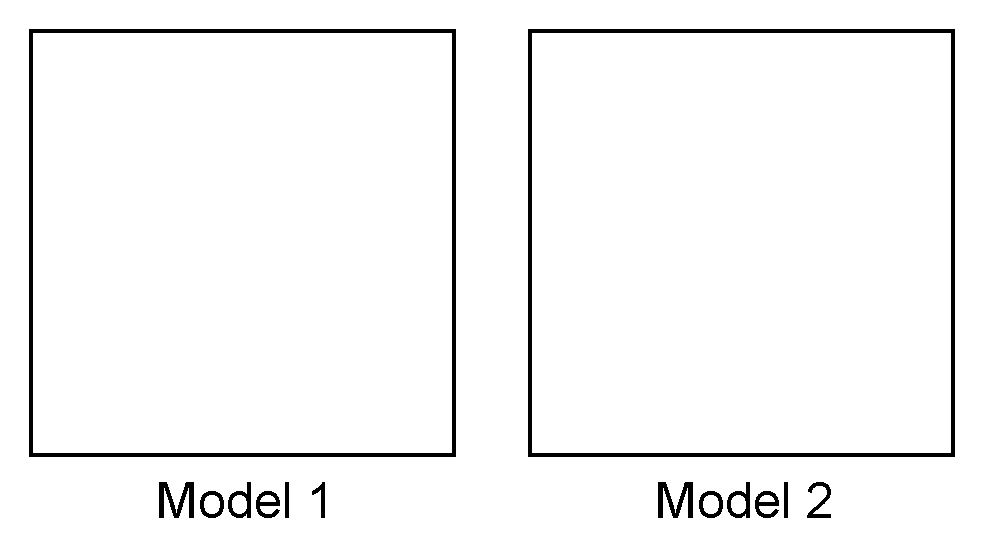
\includegraphics[width=0.75\textwidth]{\figpath/Model1and2_blank.pdf}}
		
		\item Calculate the number-average degree of polymerization for both of the ``final'' states you drew in response to the previous question:
		
		\vspace{1in}
	\end{enumerate}

\subsection{Model 3: A Stoichiometrically-Imbalanced Reaction Mixture}

Practically speaking, it is often very difficult to ensure that a reaction mixture is perfectly stoichiometrically-balanced, and there is often a small excess of one type of monomer or the other.

Consider a reaction mixture that starts with 3 AA-type monomers and 5 BB-type monomers:

\vspace{0.1in}
\centerline{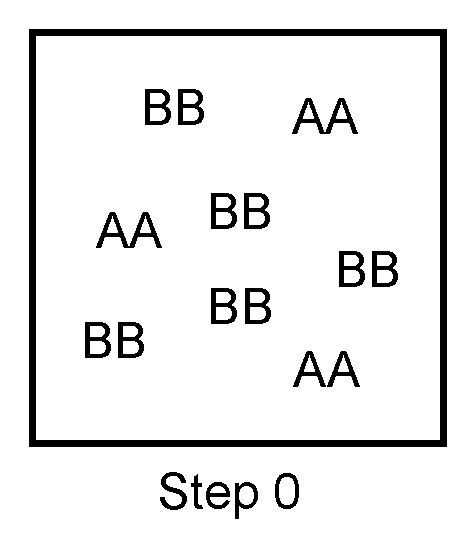
\includegraphics[width=0.9\textwidth]{\figpath/AABBpolym-nonstoich.pdf}}

\subsection*{Critical Thinking Questions}

	\begin{enumerate}[resume]
		\item Fill in the blank spaces in the model, above, with reasonable predictions for what the reaction mixture might look like in each successive step.
		
		\item Which type of reactive group is the ``limiting reagent'' in this reaction?
		
		\item \label{ctq:nonstoichpredict} Predict what the reaction mixture in Model 3 might look like if you let it react until no more reactions could take place:
		
\vspace{0.1in}
\centerline{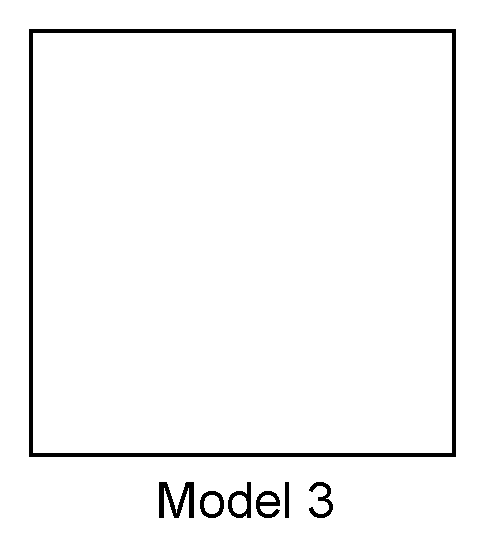
\includegraphics[width=0.3\textwidth]{\figpath/Model3_blank.pdf}}
		
		\item Calculate the number-average degree of polymerization for the ``final'' state you drew in response to the previous question:
		
		\vspace{1in}
		
		\item Is the final degree of polymerization for this stoichiometrically-unbalanced reaction smaller than, equal to, or larger than the final degree of polymerization you calculated for the stoichiometrically-balanced reactions in Models 1 and 2?
		
		\vspace{0.5in}
		
		\item Which type of reactive group is on the ends of all of the chains you drew in question \ref{ctq:nonstoichpredict}?
		
		\vspace{0.5in}
		
		\item Briefly critique or defend the following statement:
		
			\emph{``When drawing the structure of a polymer produced by a step-growth polymerization, we should always make sure that we draw end groups consistent with whichever reactive species was present in excess.''}
		
		\vspace{1in}
			
	\end{enumerate}
	
	INFORMATION: In stoichiometrically-imbalanced step-growth polymerizations with an excess of B groups, we define a parameter $r$ that reflects the ratio of A groups to B groups.	
	If the initial number of A groups is $v_A^0$ and the initial number of B groups is $v_b^0$, then
	\begin{equation*}
		r = \frac{v_A^0}{v_B^0}
	\end{equation*}
	
	
	For a reaction mixture with stoichiometric imbalance $r$ at extent of reaction $p$, the number-average degree of polymerization is given by
	\begin{equation*}
		N_n = \frac{1+r}{1+r-2pr}
	\end{equation*}
	
	\begin{enumerate}[resume]
		%\item When $r=1$, how can you simplify this expression for $N_n$?		
		%\item When $p=1$, how can you simplify this expression for $N_n$?
		\item Using this expression, fill in the following table with the expected number-average degree of polymerization for different combinations of $r$ and $p$ values:
		
			\begin{table}[!h]
				\centering
				\renewcommand{\arraystretch}{3}
				\begin{tabular}{|c|c|c|c|}
					\hline
					 &  ~$p=0.9$~ & ~$p=0.99$~ & ~$p=0.999$~ \\\hline
					$r=0.9$ &&& \\\hline
					$r=0.99$ &&& \\\hline
					$r=0.999$ &&& \\\hline
				\end{tabular}
			\end{table}
		
		\item On the basis of your answers to the previous question, briefly critique or defend the following statement:
		
			\emph{``Achieving high molecular weights in step-growth polymerizations requires both very precise measurement of the reagents, and reaction conditions which strongly favor the bond-forming reaction.''}
			
	\end{enumerate}

\subsection{Exercises}

	%After class, \textbf{read} the following sections of your textbook:
	
	%\begin{enumerate}
	%	\item First section
	%	\item Second section
	%\end{enumerate}
	
	%Then, do the following exercises:
	
	Continue with the following exercises if your group finishes the above activities before the end of class:
	
	\begin{enumerate}
		\item In this activity, we only calculated the number-average \emph{degree of polymerization} of the polymers produced in step-growth polymerizations. However, usually, we want to be able to calculate the \emph{molecular weight} of the polymers as well.
		
			\begin{enumerate}
				\item In Model 1, we considered a reaction of AB-type monomers.  If each monomer had mass $m_{AB}$, how would you calculate the number-average molecular weight, $M_n$, of the polymer produced when the extent of reaction is equal to $p$?
				
				\item In Model 2, we considered a stoichiometrically-balanced reaction of AA- and BB-type monomers. If the AA-type monomers each had mass $m_{AA}$ and the BB-type monomers each had mass $m_{BB}$, how would you calculate the number-average molecular weight of the polymer produced when the extent of reaction is equal to $p$?
				
					\emph{Note: this question is a little tricky - remember that $N_n$ counts \emph{monomers}, but in this reaction, not all of the monomers have the same molecular weight.  How might you be able to correct for this?}
				
			\end{enumerate}
		
		\item In Model 3, we considered a stoichiometrically-imbalanced reaction of AA- and BB-type monomers.  However, another important limit occurs when we have equal numbers of AA- and BB-type monomers, but add in an extra monofunctional reagent ``Bx'' that can only react on one side.
		
			\begin{enumerate}
				\item How many ``Bx'' molecules would you need to add to the reaction mixture to have the same number of extra ``B'' groups as you would get from a single extra BB-type monomer?
				
				\item (Modify stoich imbalance eqn to reflect this case?)
				
				\item Monofunctional reagents are a common impurity in supplies of difunctional monomers. Briefly explain why this means it is necessary to rigorously purify the starting materials used in step-growth polymerizations.
			\end{enumerate}
	\end{enumerate}